\documentclass{article}
\usepackage[utf8]{inputenc}
\usepackage{authblk}
\usepackage{hyperref}
\usepackage[title]{appendix}
\usepackage{graphicx}
\usepackage{subfloat}





\title{PhD Training Short Course \\ Time-series Econometrics \\ Assignment}
\author[1]{Stylianos Zlatanos\thanks{King's Business School, King's College London; \href{mailto:stylianos.zlatanos@kcl.ac.uk}{stylianos.zlatanos@kcl.ac.uk}}}
\date{\today}

\begin{document}

\maketitle

\section{Question 1: Monte Carlo}
\paragraph{$AR(1)$ model}
\begin{enumerate}
    \item 
    \begin{enumerate}
        \item Mean \\ \textit{Considering different samples}
        
        \par
        \textit{Considering different autoregressive parameters}
        
         \par
        \textit{Considering different autoregressive parameters}
        
        \item Variance \\ \textit{Considering different samples}
        
        \par
        \textit{Considering different autoregressive parameters}
        
         \par
        \textit{Considering different autoregressive parameters}
        
        \item $AR$ coefficients \\ \textit{Considering different samples}
        
        \par
        \textit{Considering different autoregressive parameters}
        
         \par
        \textit{Considering different autoregressive parameters}
        
    \end{enumerate}
\end{enumerate}


\paragraph{$MA(1)$ model}
\begin{enumerate}
    \item 
    \begin{enumerate}
        \item Mean \\ \textit{Considering different samples}
        
        \par
        \textit{Considering different autoregressive parameters}
        
         \par
        \textit{Considering different autoregressive parameters}
        
        \item Variance \\ \textit{Considering different samples}
        
        \par
        \textit{Considering different autoregressive parameters}
        
         \par
        \textit{Considering different autoregressive parameters}
        
        \item $AR$ coefficients \\ \textit{Considering different samples}
        
        \par
        \textit{Considering different autoregressive parameters}
        
         \par
        \textit{Considering different autoregressive parameters}
        
    \end{enumerate}
\end{enumerate}


\section{Question 2: Block Bootstrap}
\section{Question 3: Sparse Regression and Factor Analysis}


\clearpage
\appendix
\section{Figures}
%%%%%%%%%%%%%%%%%%%%%%
\subsection{Monte Carlo}
\subsubsection{$AR(1)$ models}
\begin{figure}[hbt!]
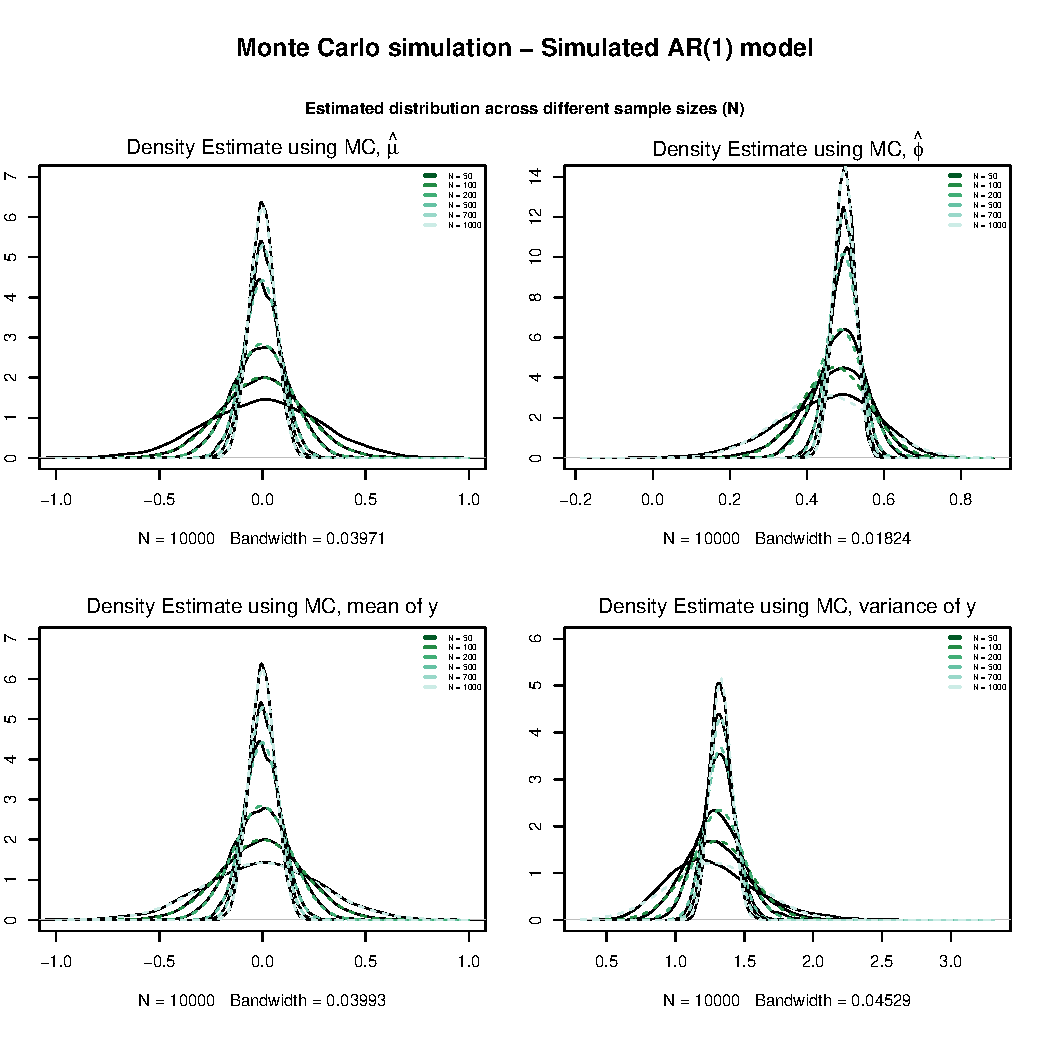
\includegraphics[width=\textwidth]{plots/MC_AR1_densities_diff_smpl}
\label{fig:MC_AR1_densities_diff_smpl}
\caption{MC simulation for an $AR(1)$ model: changing the sample size}
\centering
\end{figure}

\begin{figure}[hbt!]
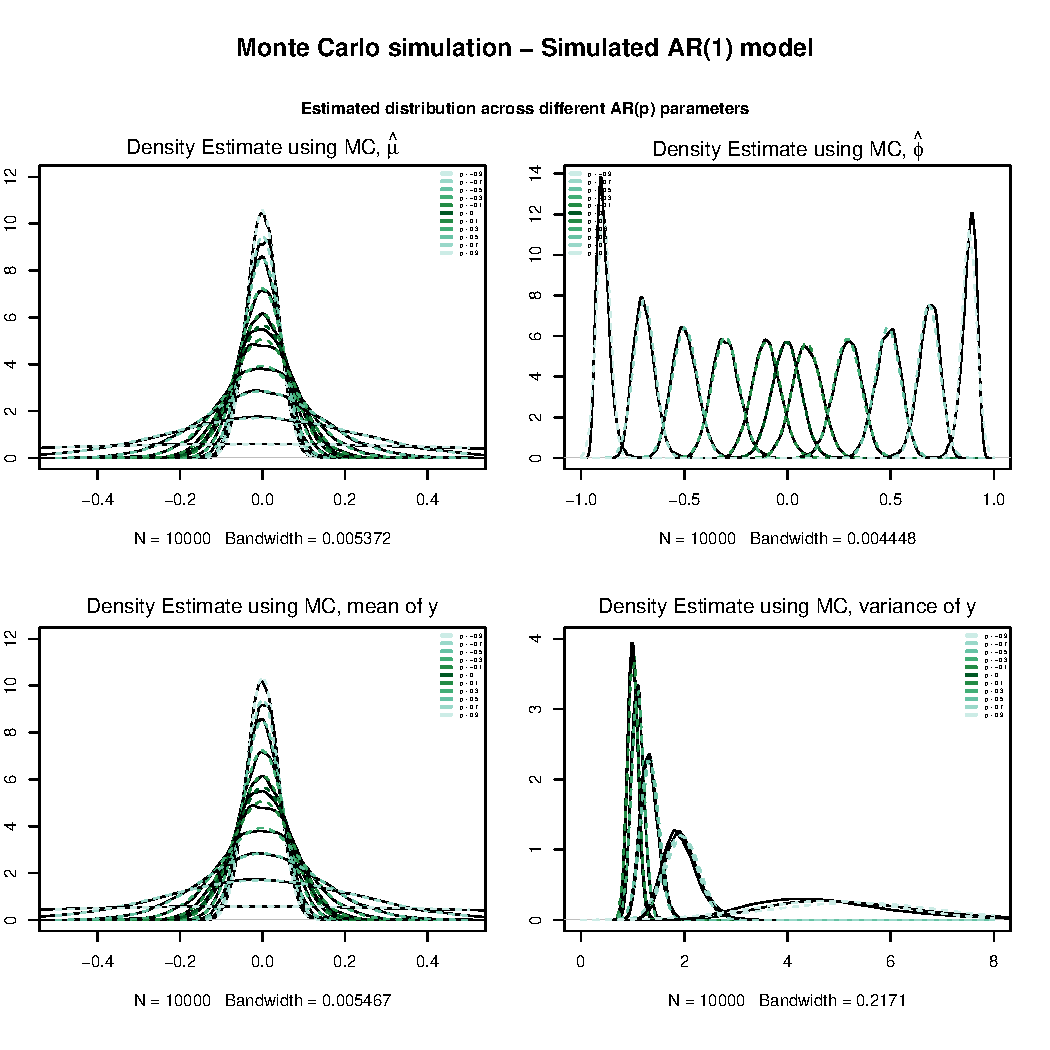
\includegraphics[width=\textwidth]{plots/MC_AR1_densities_diff_ARq}
\label{fig:MC_AR1_densities_diff_ARq}
\caption{MC simulation for an $AR(1)$ model: changing the autoregressive parameter}
\centering
\end{figure}

\begin{figure}[hbt!]
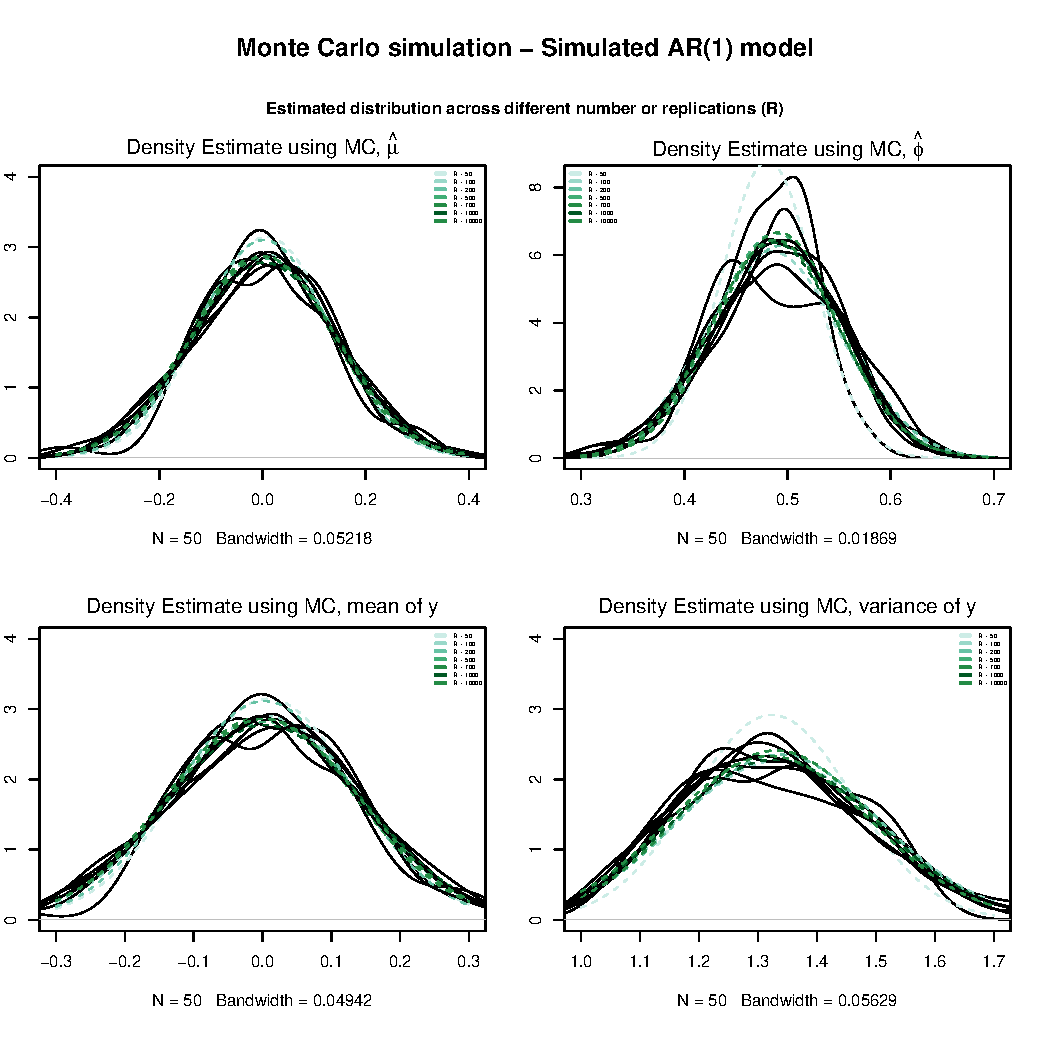
\includegraphics[width=\textwidth]{plots/MC_AR1_densities_diff_norepl}
\label{fig:MC_AR1_densities_diff_norepl}
\caption{MC simulation for an $AR(1)$ model: changing the number of replications}
\centering
\end{figure}


\clearpage
\subsubsection{$MA(1)$ models}
\begin{figure}[hbt!]
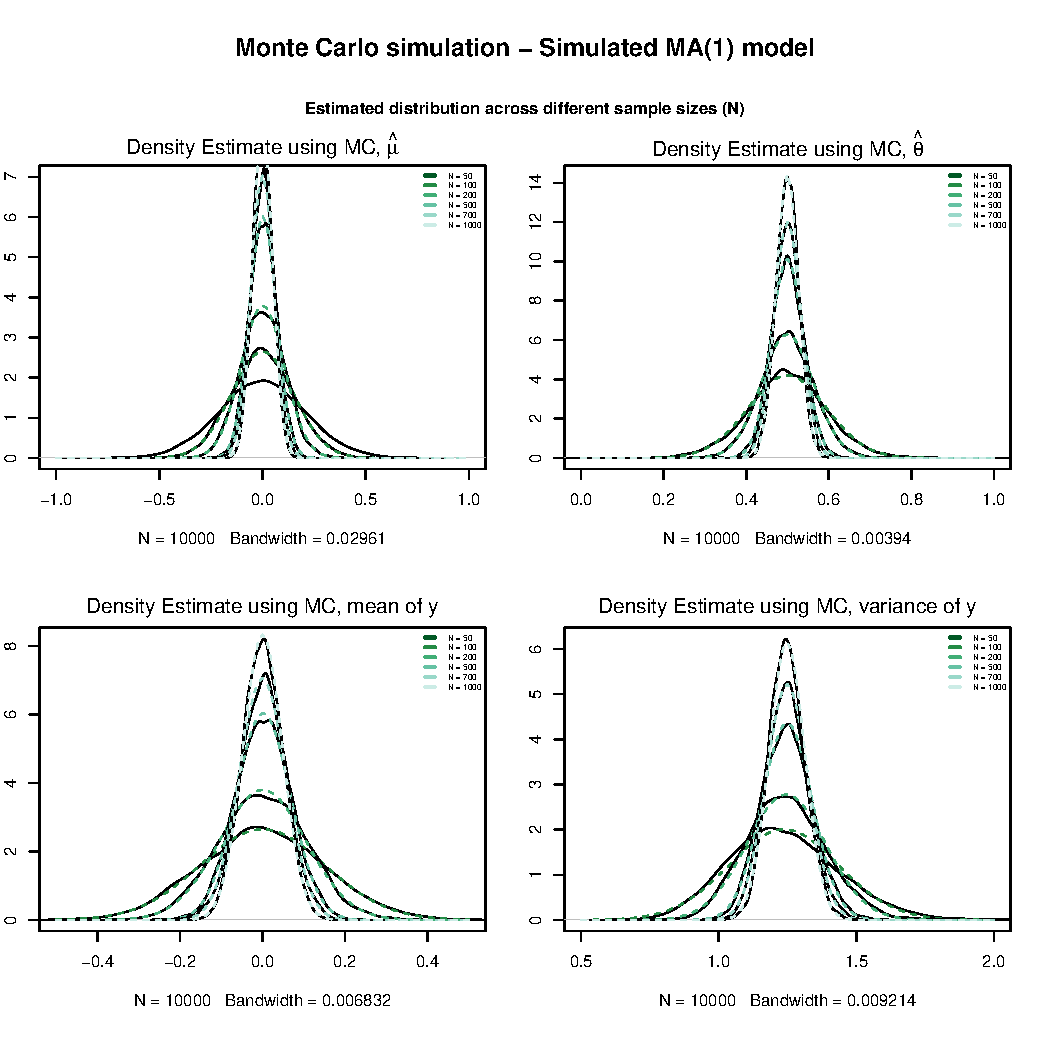
\includegraphics[width=\textwidth]{plots/MC_MA1_densities_diff_smpl}
\label{fig:MC_MA1_densities_diff_smpl}
\caption{MC simulation for an $MA(1)$ model: changing the sample size}
\centering
\end{figure}

\begin{figure}[hbt!]
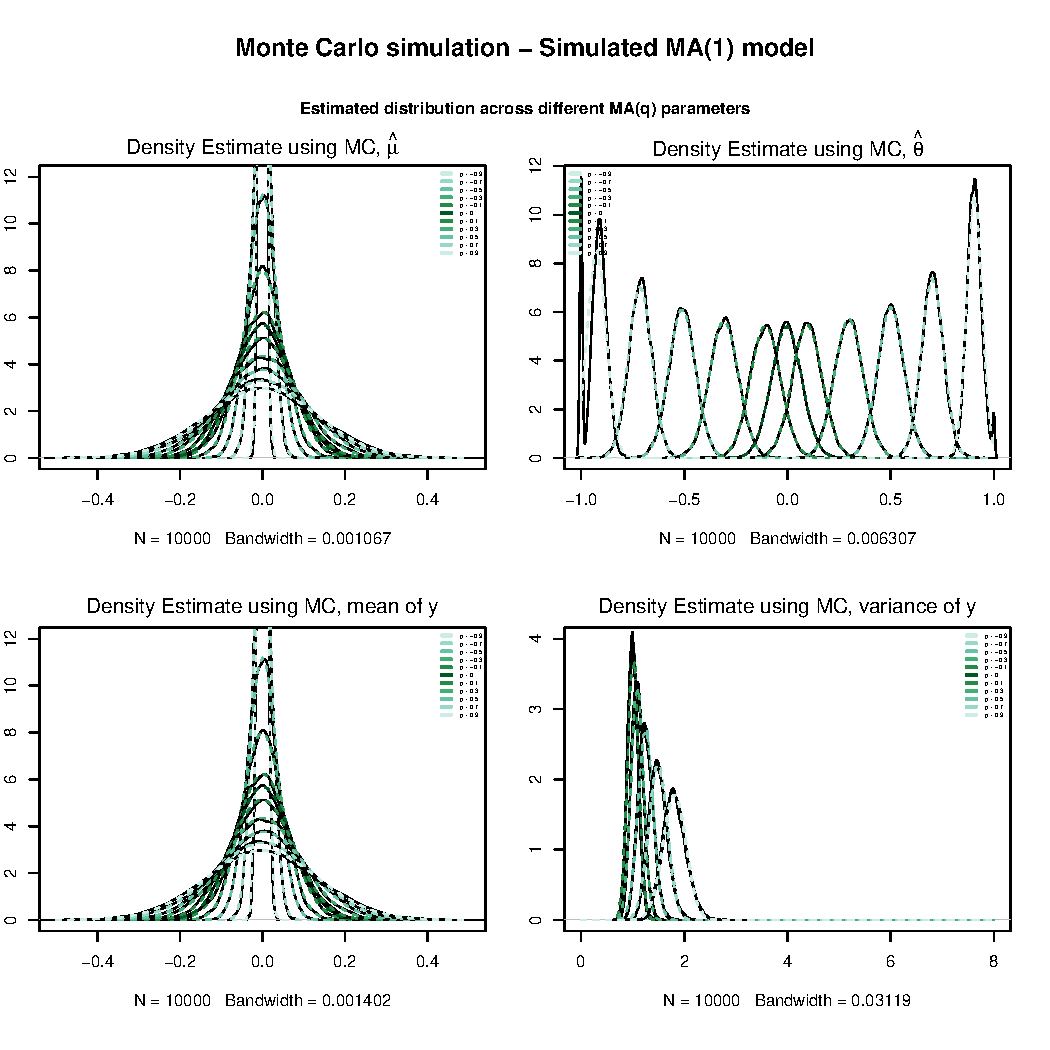
\includegraphics[width=\textwidth]{plots/MC_MA1_densities_diff_ARq}
\label{fig:MC_MA1_densities_diff_ARq}
\caption{MC simulation for an $MA(1)$ model: changing the autoregressive parameter}
\centering
\end{figure}

\begin{figure}[hbt!]
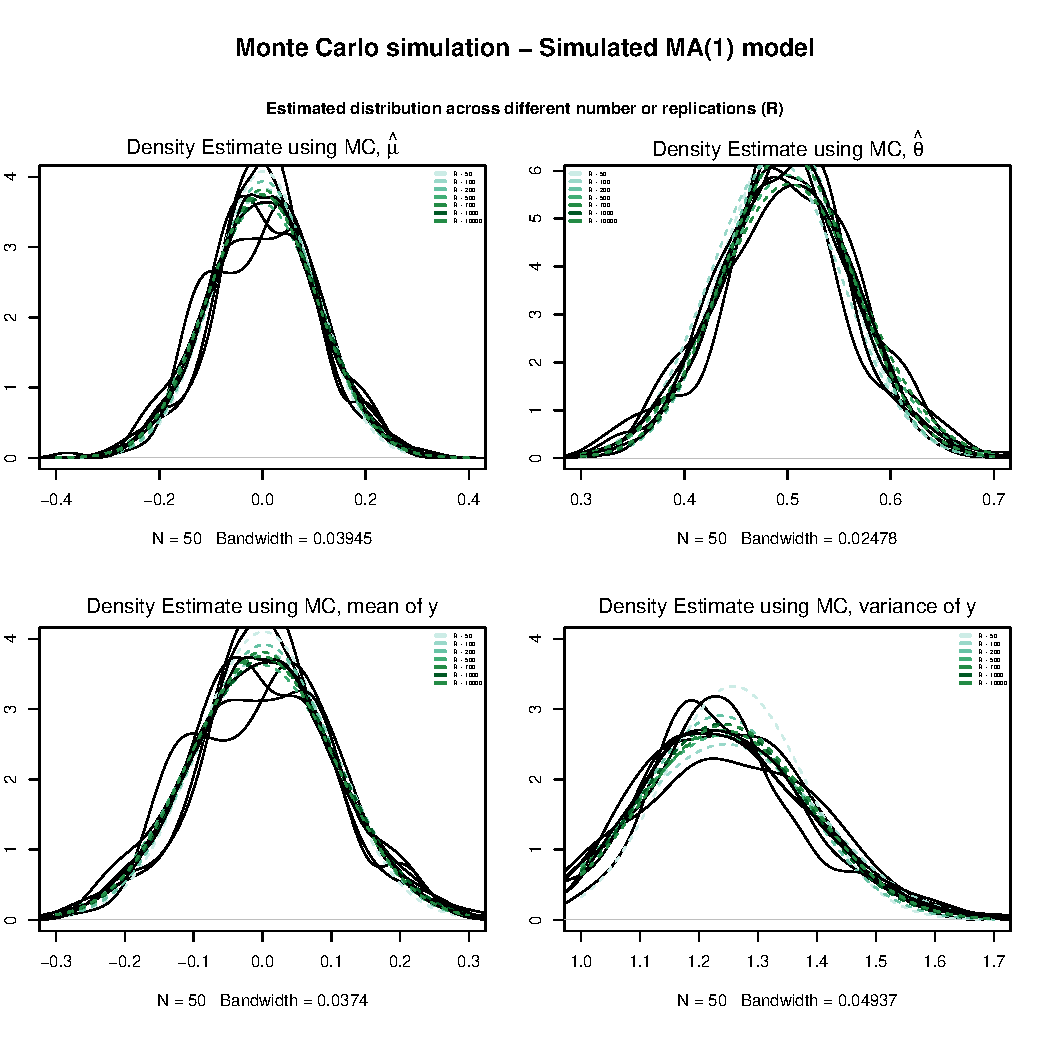
\includegraphics[width=\textwidth]{plots/MC_MA1_densities_diff_norepl}
\label{fig:MC_MA1_densities_diff_norepl}
\caption{MC simulation for an $MA(1)$ model: changing the number of replications}
\centering
\end{figure}



\clearpage
%%%%%%%%%%%%%%%%%%%%%%
\subsection{Moving Block Bootstrap}
\subsubsection{$AR(1)$ models}
\begin{figure}[hbt!]
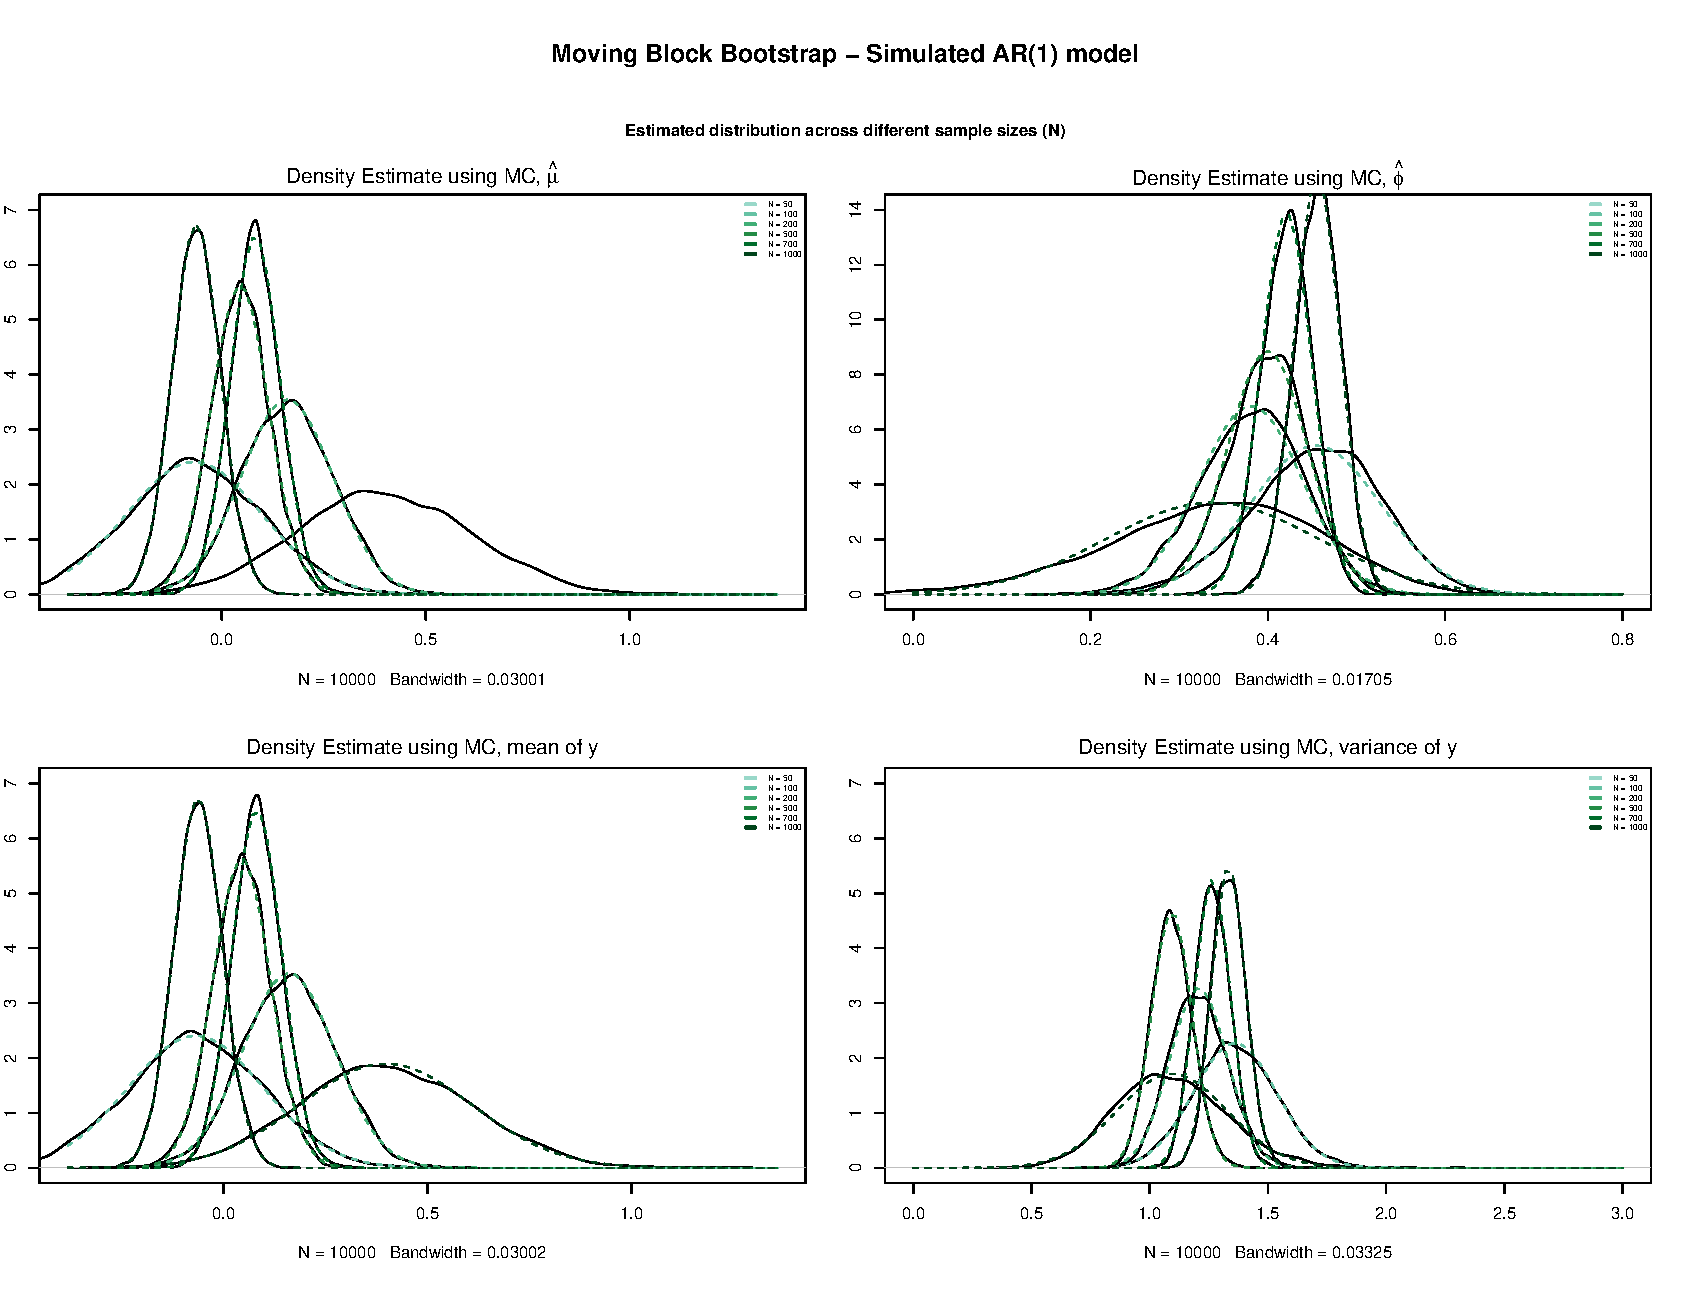
\includegraphics[width=\textwidth]{plots/MBB_AR1_densities_diff_smpl}
\label{fig:MBB_AR1_densities_diff_smpl}
\caption{MBB for an $AR(1)$ model: changing the sample size}
\centering
\end{figure}

\begin{figure}[hbt!]
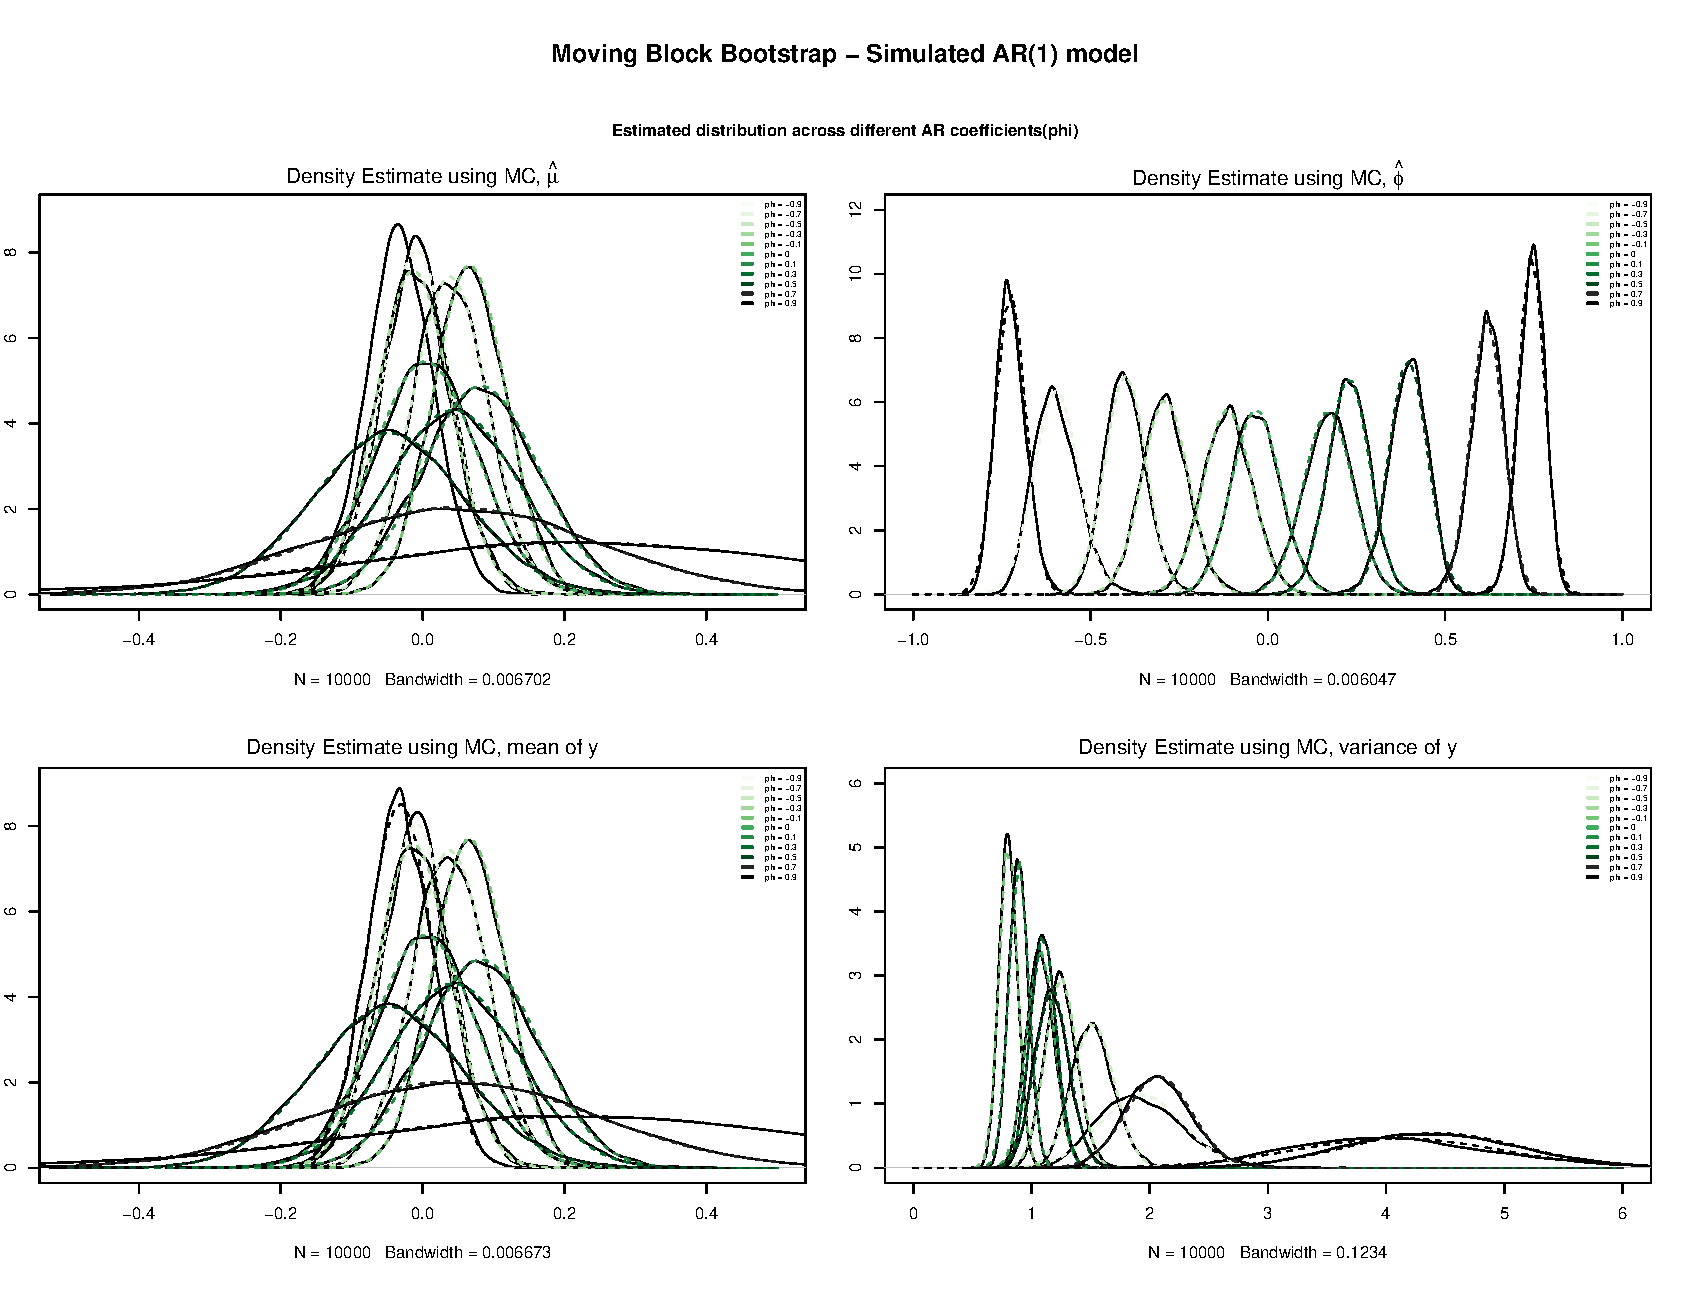
\includegraphics[width=\textwidth]{plots/MBB_AR1_densities_diff_ARq}
\label{fig:MBB_AR1_densities_diff_ARq}
\caption{MBB for an $AR(1)$ model: changing the autoregressive parameter}
\centering
\end{figure}

\begin{figure}[hbt!]
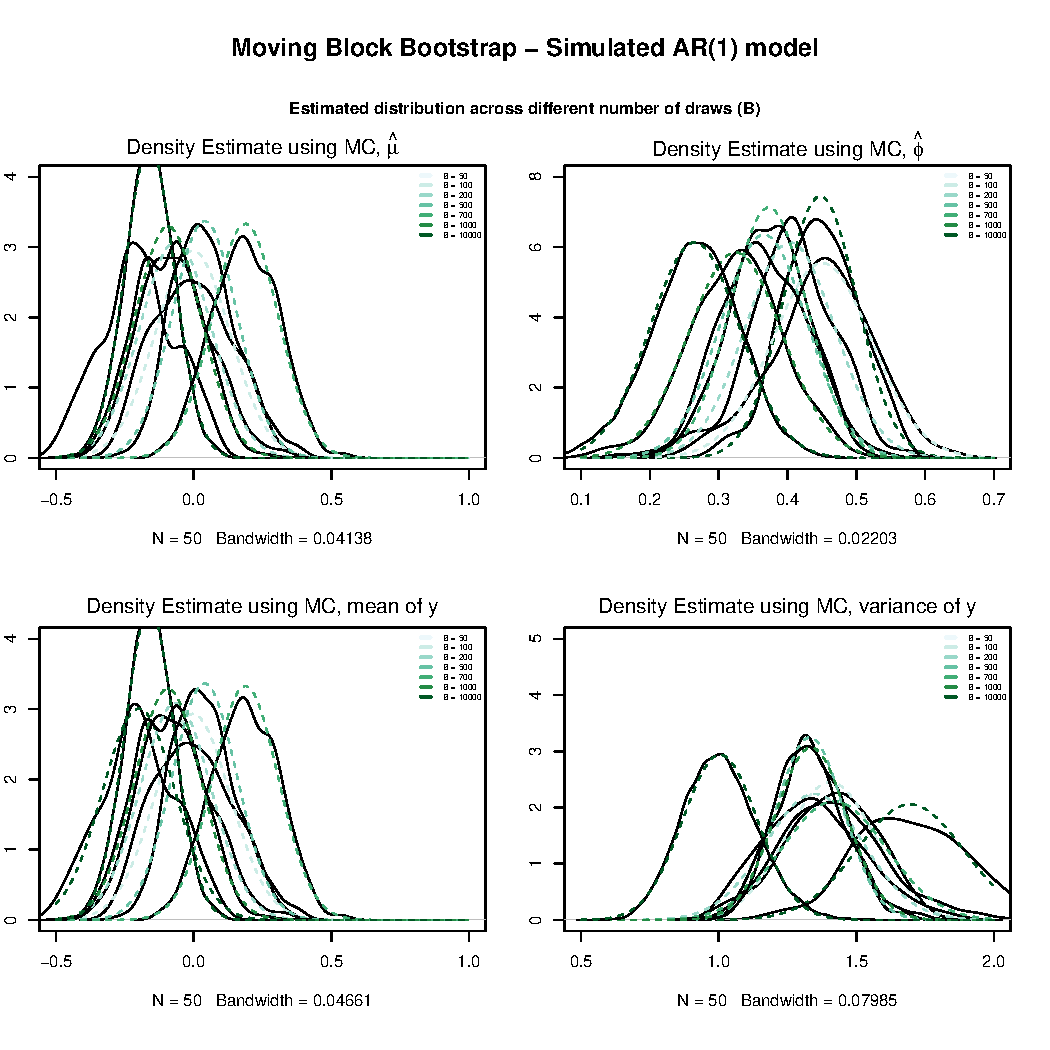
\includegraphics[width=\textwidth]{plots/MBB_AR1_densities_diff_drawsB}
\label{fig:MBB_AR1_densities_diff_drawsB}
\caption{MBB for an $AR(1)$ model: changing the number of draws}
\centering
\end{figure}

\begin{figure}[hbt!]
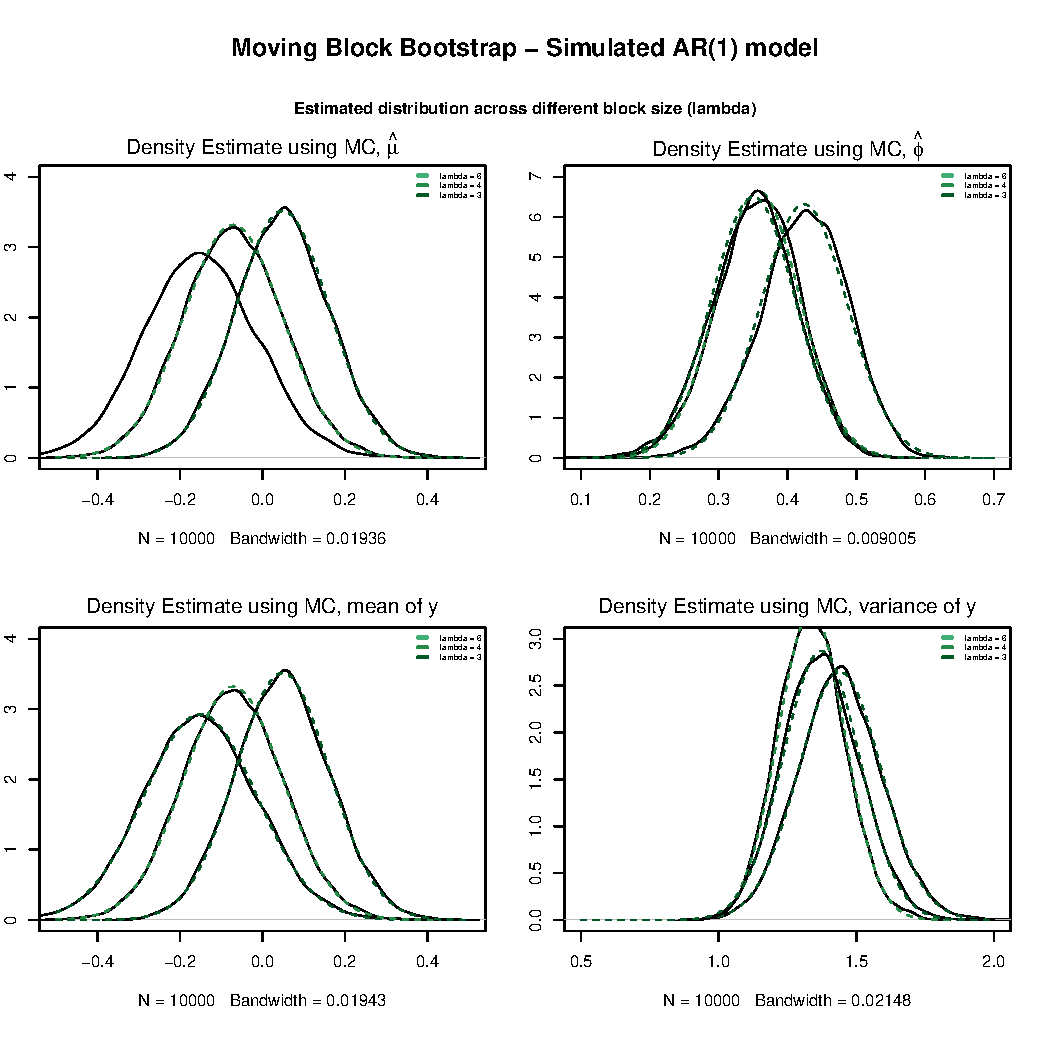
\includegraphics[width=\textwidth]{plots/MBB_AR1_densities_diff_blocklength}
\label{fig:MBB_AR1_densities_diff_blocklength}
\caption{MBB for an $AR(1)$ model: changing the block length}
\centering
\end{figure}


\clearpage
\subsubsection{$MA(1)$ models}
\begin{figure}[hbt!]
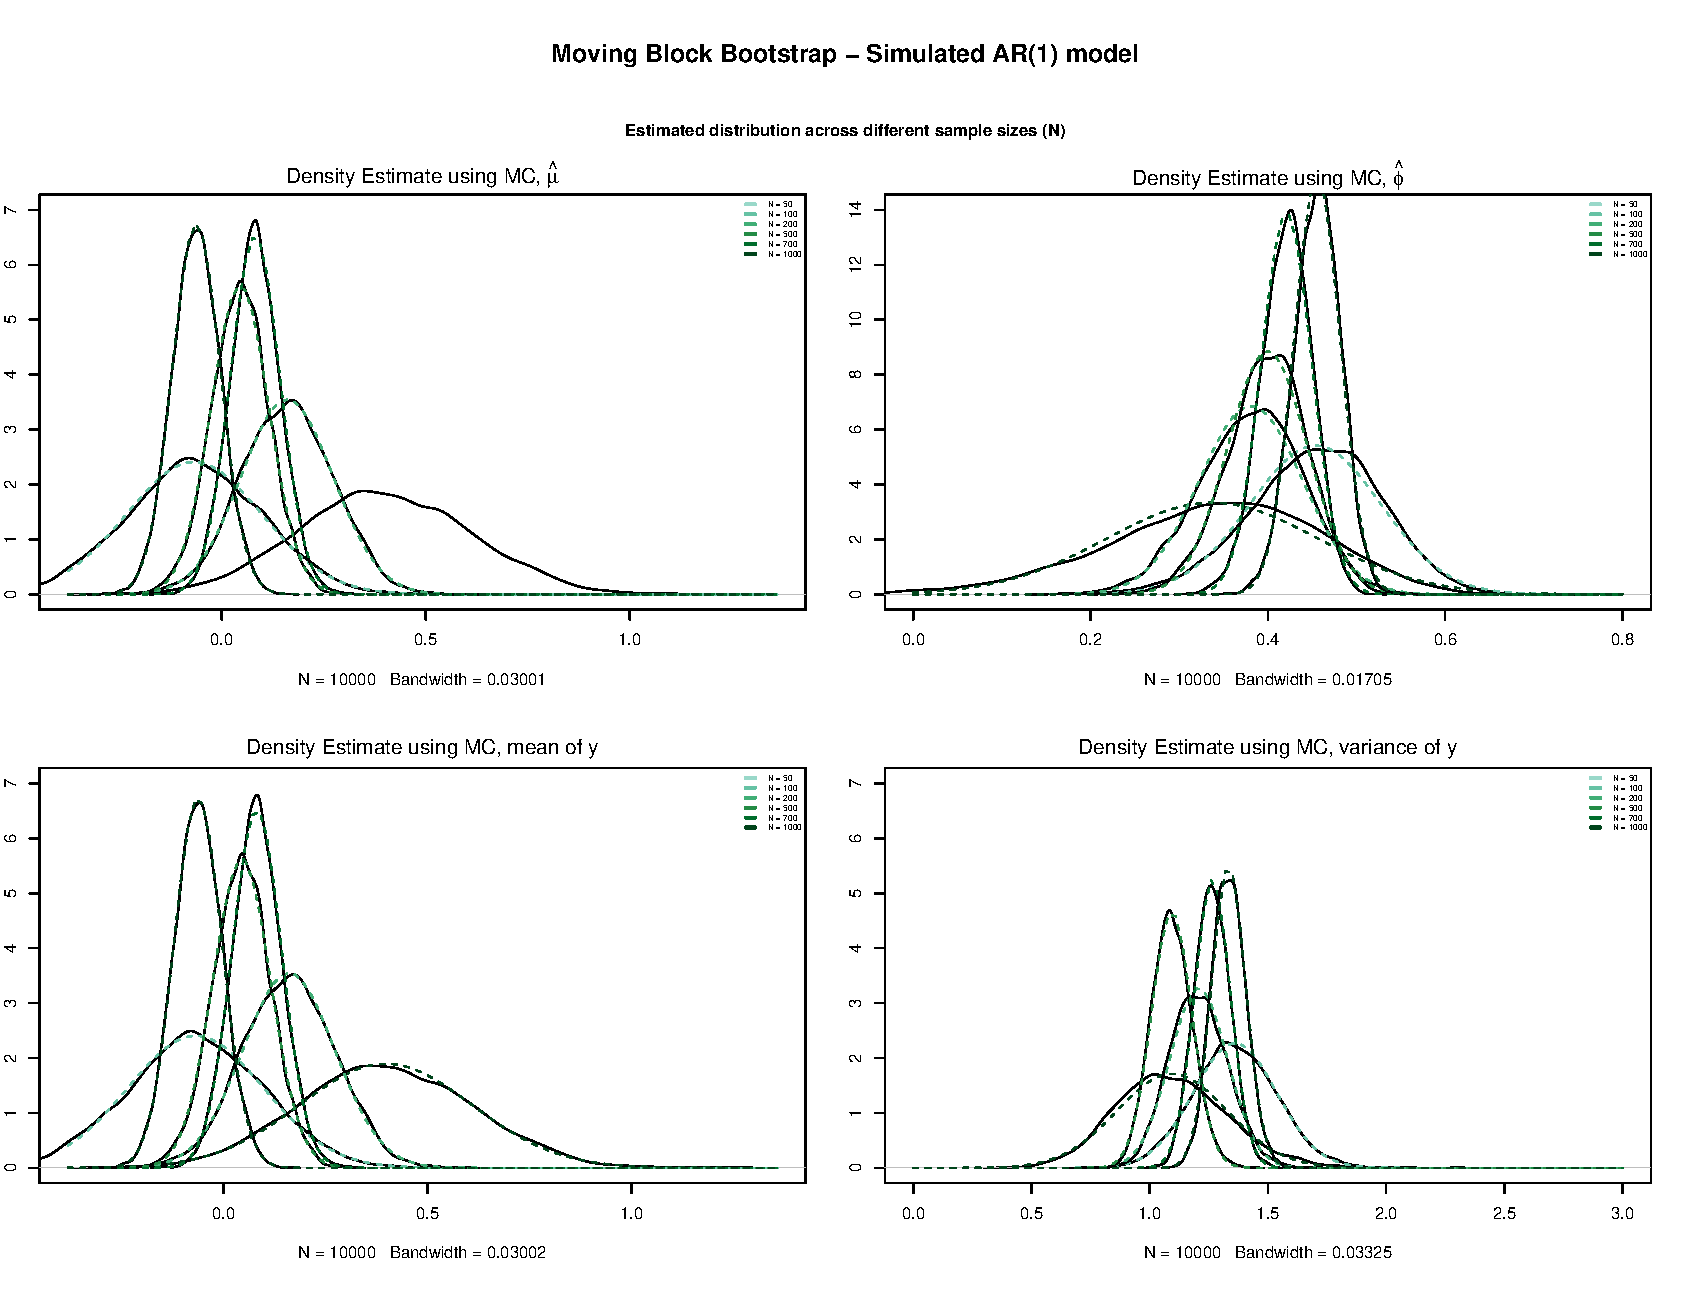
\includegraphics[width=\textwidth]{plots/MBB_AR1_densities_diff_smpl}
\label{fig:MBB_MA1_densities_diff_smpl}
\caption{MBB for an $MA(1)$ model: changing the sample size}
\centering
\end{figure}

\begin{figure}[hbt!]
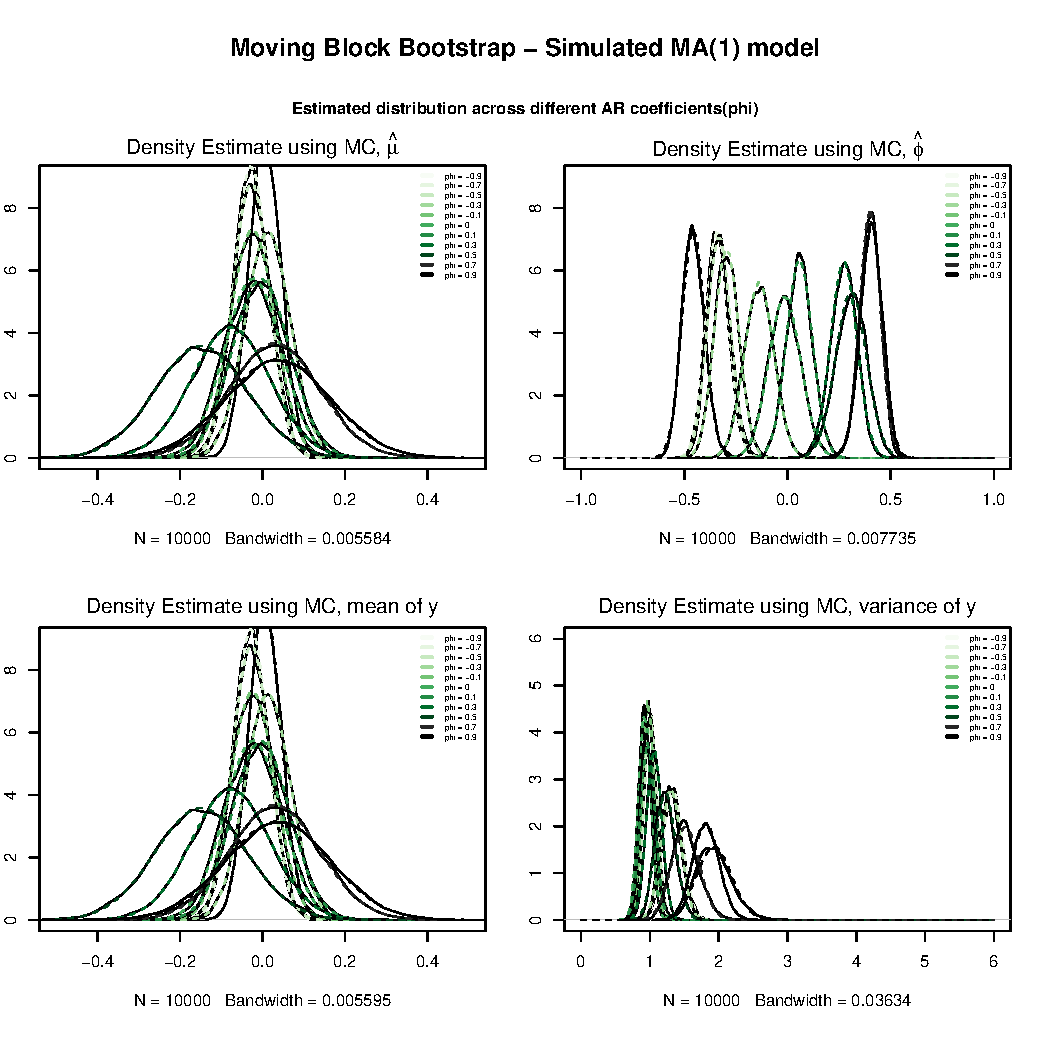
\includegraphics[width=\textwidth]{plots/MBB_MA1_densities_diff_ARq}
\label{fig:MBB_MA1_densities_diff_ARq}
\caption{MBB for an $MA(1)$ model: changing the autoregressive parameter}
\centering
\end{figure}

\begin{figure}[hbt!]
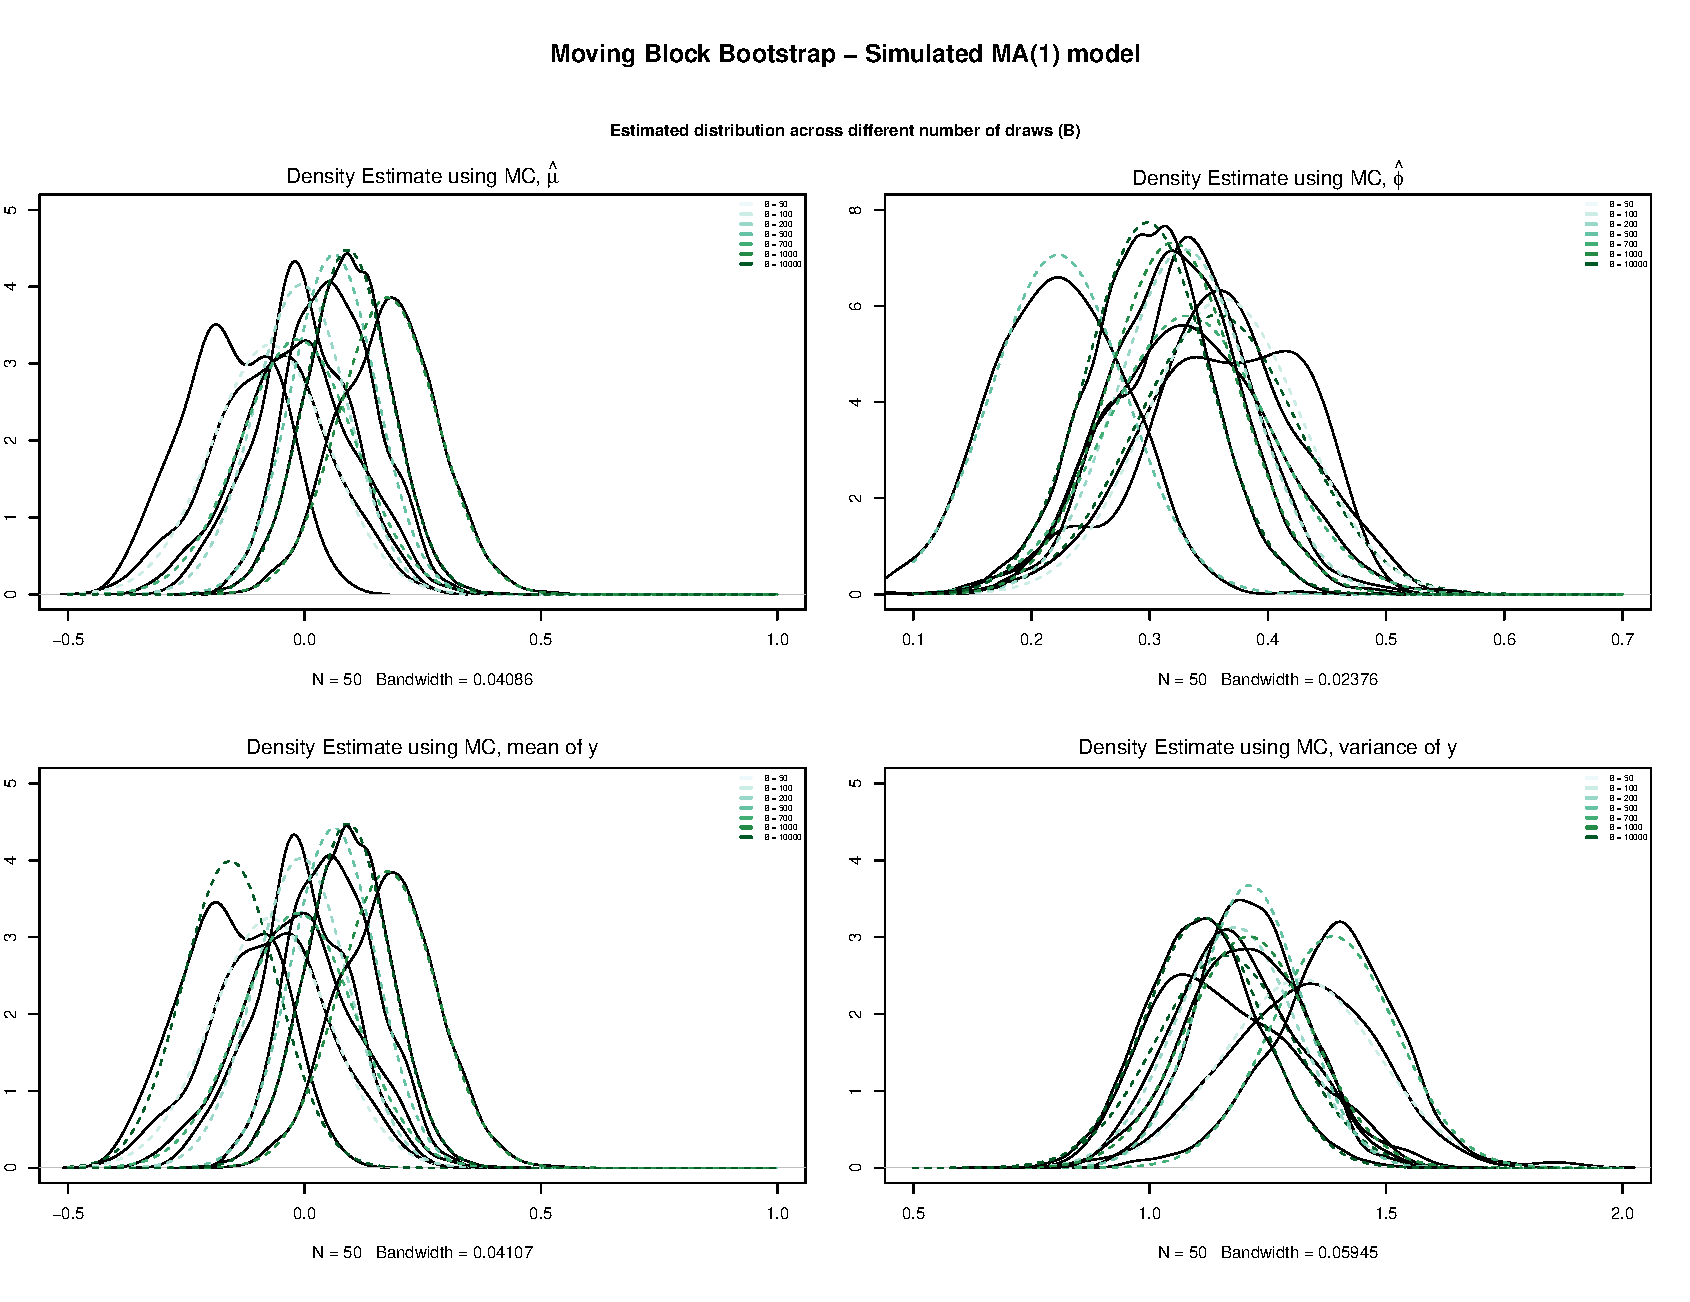
\includegraphics[width=\textwidth]{plots/MBB_MA1_densities_diff_drawsB}
\label{fig:MBB_MA1_densities_diff_drawsB}
\caption{MBB for an $MA(1)$ model: changing the number of draws}
\centering
\end{figure}

\begin{figure}[hbt!]
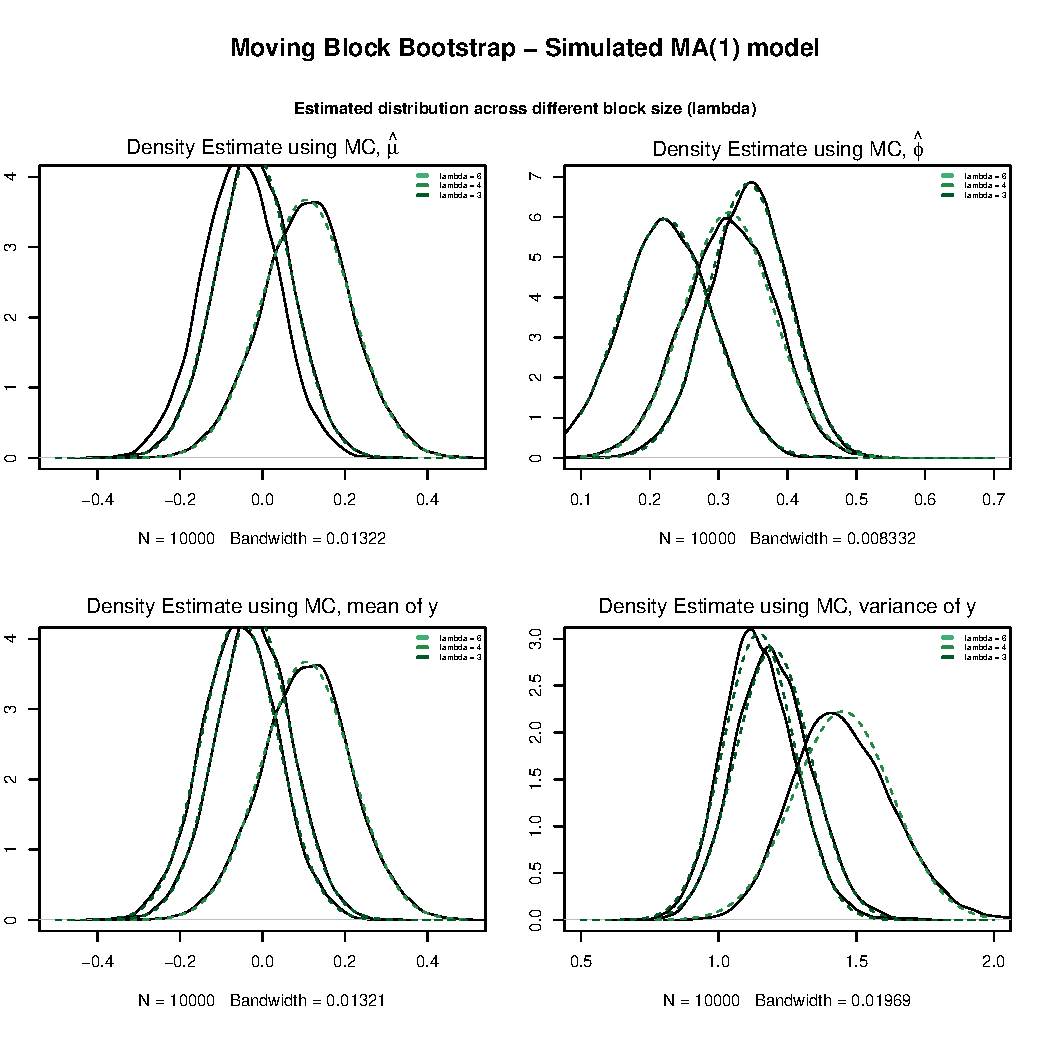
\includegraphics[width=\textwidth]{plots/MBB_MA1_densities_diff_blocklength}
\label{fig:MBB_MA1_densities_diff_blocklength}
\caption{MBB for an $MA(1)$ model: changing the block length}
\centering
\end{figure}

\clearpage
%%%%%%%%%%%%%%%%%%%%%%
\subsection{Sparse Regression and Factor Analysis}

\subsubsection{Ridge}

\begin{subfigures}
\begin{figure}[hbt!]
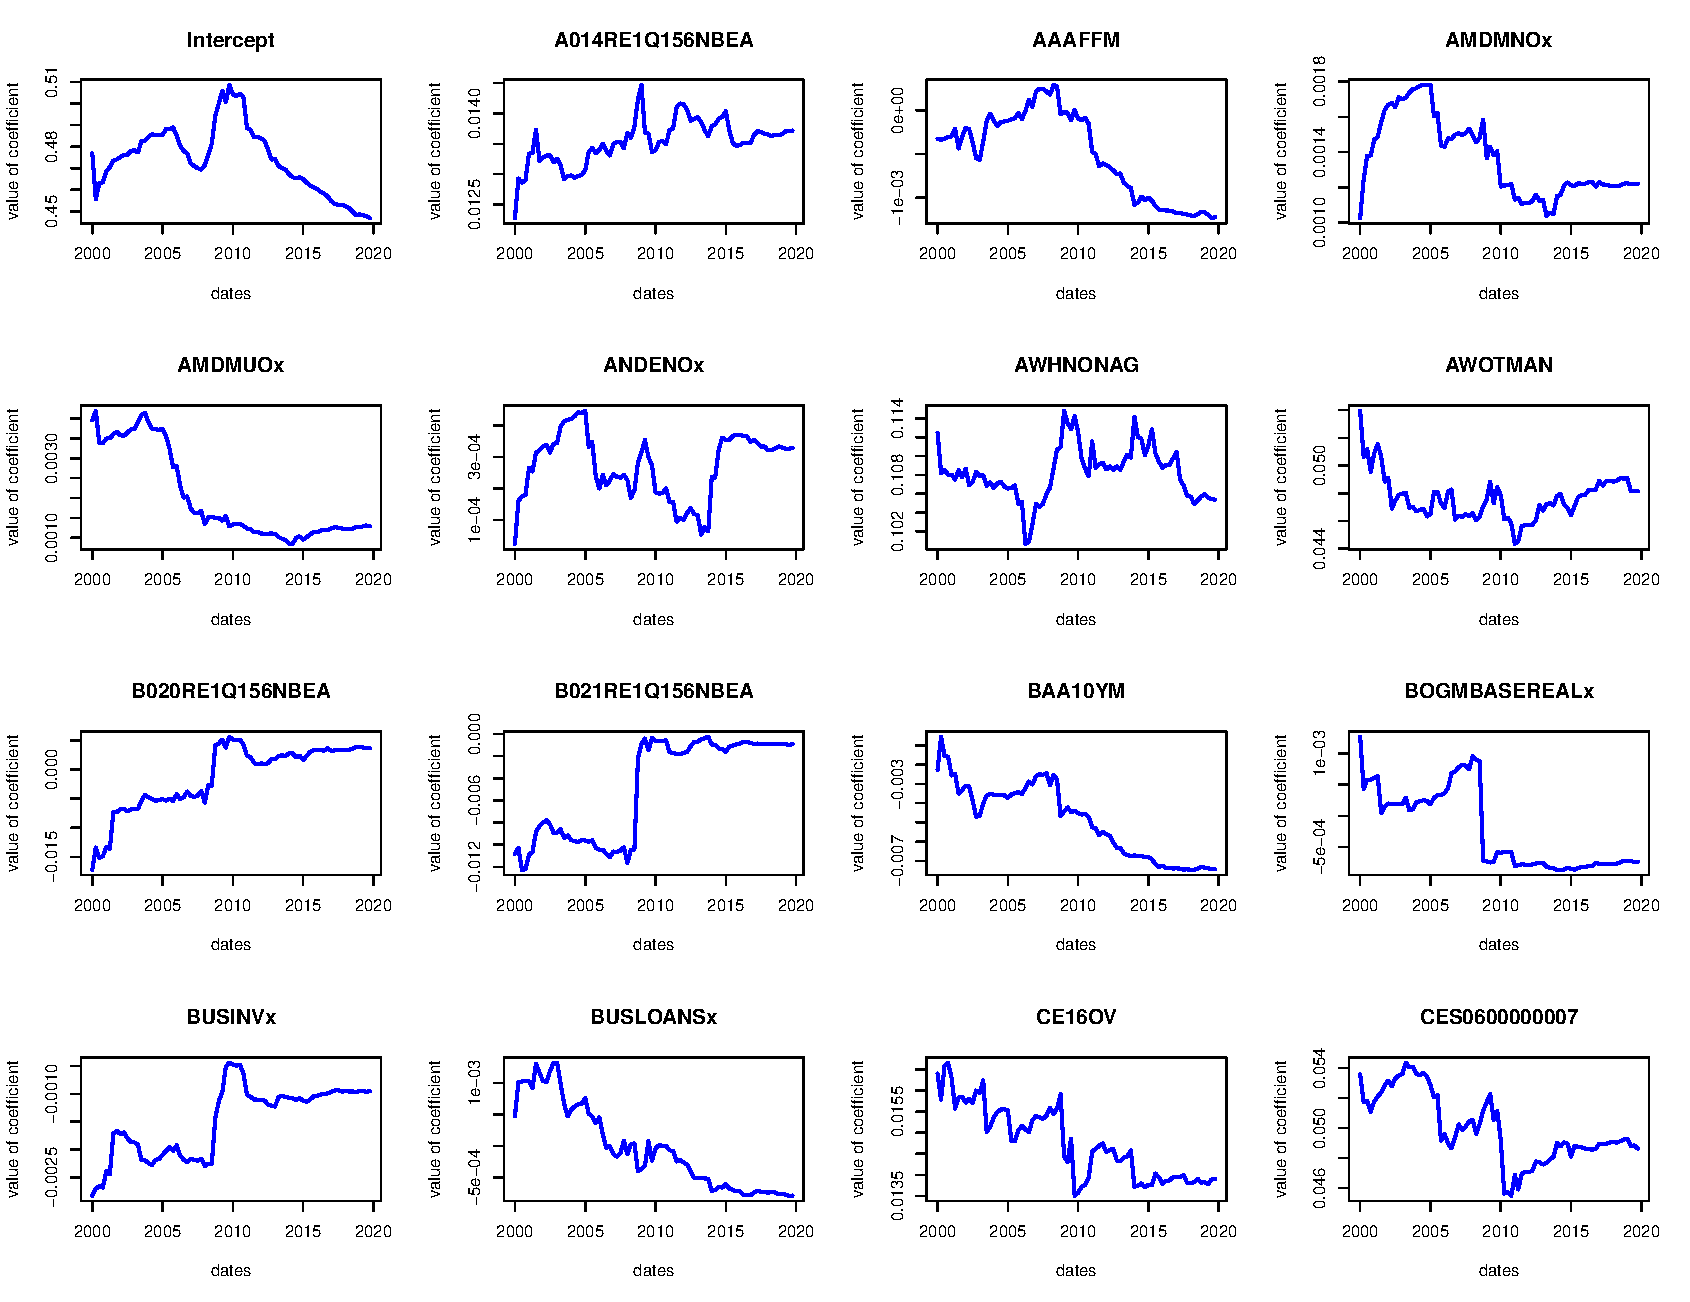
\includegraphics[page = 1, width=\textwidth]{plots/ridge_betas}
\label{fig:ridge_betas}
\caption{\label{first}Ridge regression: The evolution of the estimated $\beta$ coefficients over time}
\centering
\end{figure}

\begin{figure}[hbt!]
\includegraphics[page = 2, width=\textwidth]{plots/ridge_betas}
\label{fig:ridge_betas}
\caption{\label{second}Ridge regression: The evolution of the estimated $\beta$ coefficients over time}
\centering
\end{figure}

\begin{figure}[hbt!]
\includegraphics[page = 3, width=\textwidth]{plots/ridge_betas}
\label{fig:ridge_betas}
\caption{\label{third}Ridge regression: The evolution of the estimated $\beta$ coefficients over time}
\centering
\end{figure}

\begin{figure}[hbt!]
\includegraphics[page = 4, width=\textwidth]{plots/ridge_betas}
\label{fig:ridge_betas}
\caption{\label{fourth}Ridge regression: The evolution of the estimated $\beta$ coefficients over time}
\centering
\end{figure}

\begin{figure}[hbt!]
\includegraphics[page = 5, width=\textwidth]{plots/ridge_betas}
\label{fig:ridge_betas}
\caption{\label{fifth}Ridge regression: The evolution of the estimated $\beta$ coefficients over time}
\centering
\end{figure}

\begin{figure}[hbt!]
\includegraphics[page = 6, width=\textwidth]{plots/ridge_betas}
\label{fig:ridge_betas}
\caption{\label{sixth}Ridge regression: The evolution of the estimated $\beta$ coefficients over time}
\centering
\end{figure}

\begin{figure}[hbt!]
\includegraphics[page = 7, width=\textwidth]{plots/ridge_betas}
\label{fig:ridge_betas}
\caption{\label{seventh}Ridge regression: The evolution of the estimated $\beta$ coefficients over time}
\centering
\end{figure}

\begin{figure}[hbt!]
\includegraphics[page = 8, width=\textwidth]{plots/ridge_betas}
\label{fig:ridge_betas}
\caption{\label{eighth}Ridge regression: The evolution of the estimated $\beta$ coefficients over time}
\centering
\end{figure}

\begin{figure}[hbt!]
\includegraphics[page = 9, width=\textwidth]{plots/ridge_betas}
\label{fig:ridge_betas}
\caption{\label{ninth}Ridge regression: The evolution of the estimated $\beta$ coefficients over time}
\centering
\end{figure}

\begin{figure}[hbt!]
\includegraphics[page = 10, width=\textwidth]{plots/ridge_betas}
\label{fig:ridge_betas}
\caption{\label{tenth}Ridge regression: The evolution of the estimated $\beta$ coefficients over time}
\centering
\end{figure}

\begin{figure}[hbt!]
\includegraphics[page = 11, width=\textwidth]{plots/ridge_betas}
\label{fig:ridge_betas}
\caption{\label{eleventh}Ridge regression: The evolution of the estimated $\beta$ coefficients over time}
\centering
\end{figure}

\begin{figure}[hbt!]
\includegraphics[page = 12, width=\textwidth]{plots/ridge_betas}
\label{fig:ridge_betas}
\caption{\label{twelveth}Ridge regression: The evolution of the estimated $\beta$ coefficients over time}
\centering
\end{figure}

\begin{figure}[hbt!]
\includegraphics[page = 13, width=\textwidth]{plots/ridge_betas}
\label{fig:ridge_betas}
\caption{\label{thirteenth}Ridge regression: The evolution of the estimated $\beta$ coefficients over time}
\centering
\end{figure}


\end{subfigures}



\clearpage
\subsubsection{Lasso}

\begin{subfigures}
\begin{figure}[hbt!]
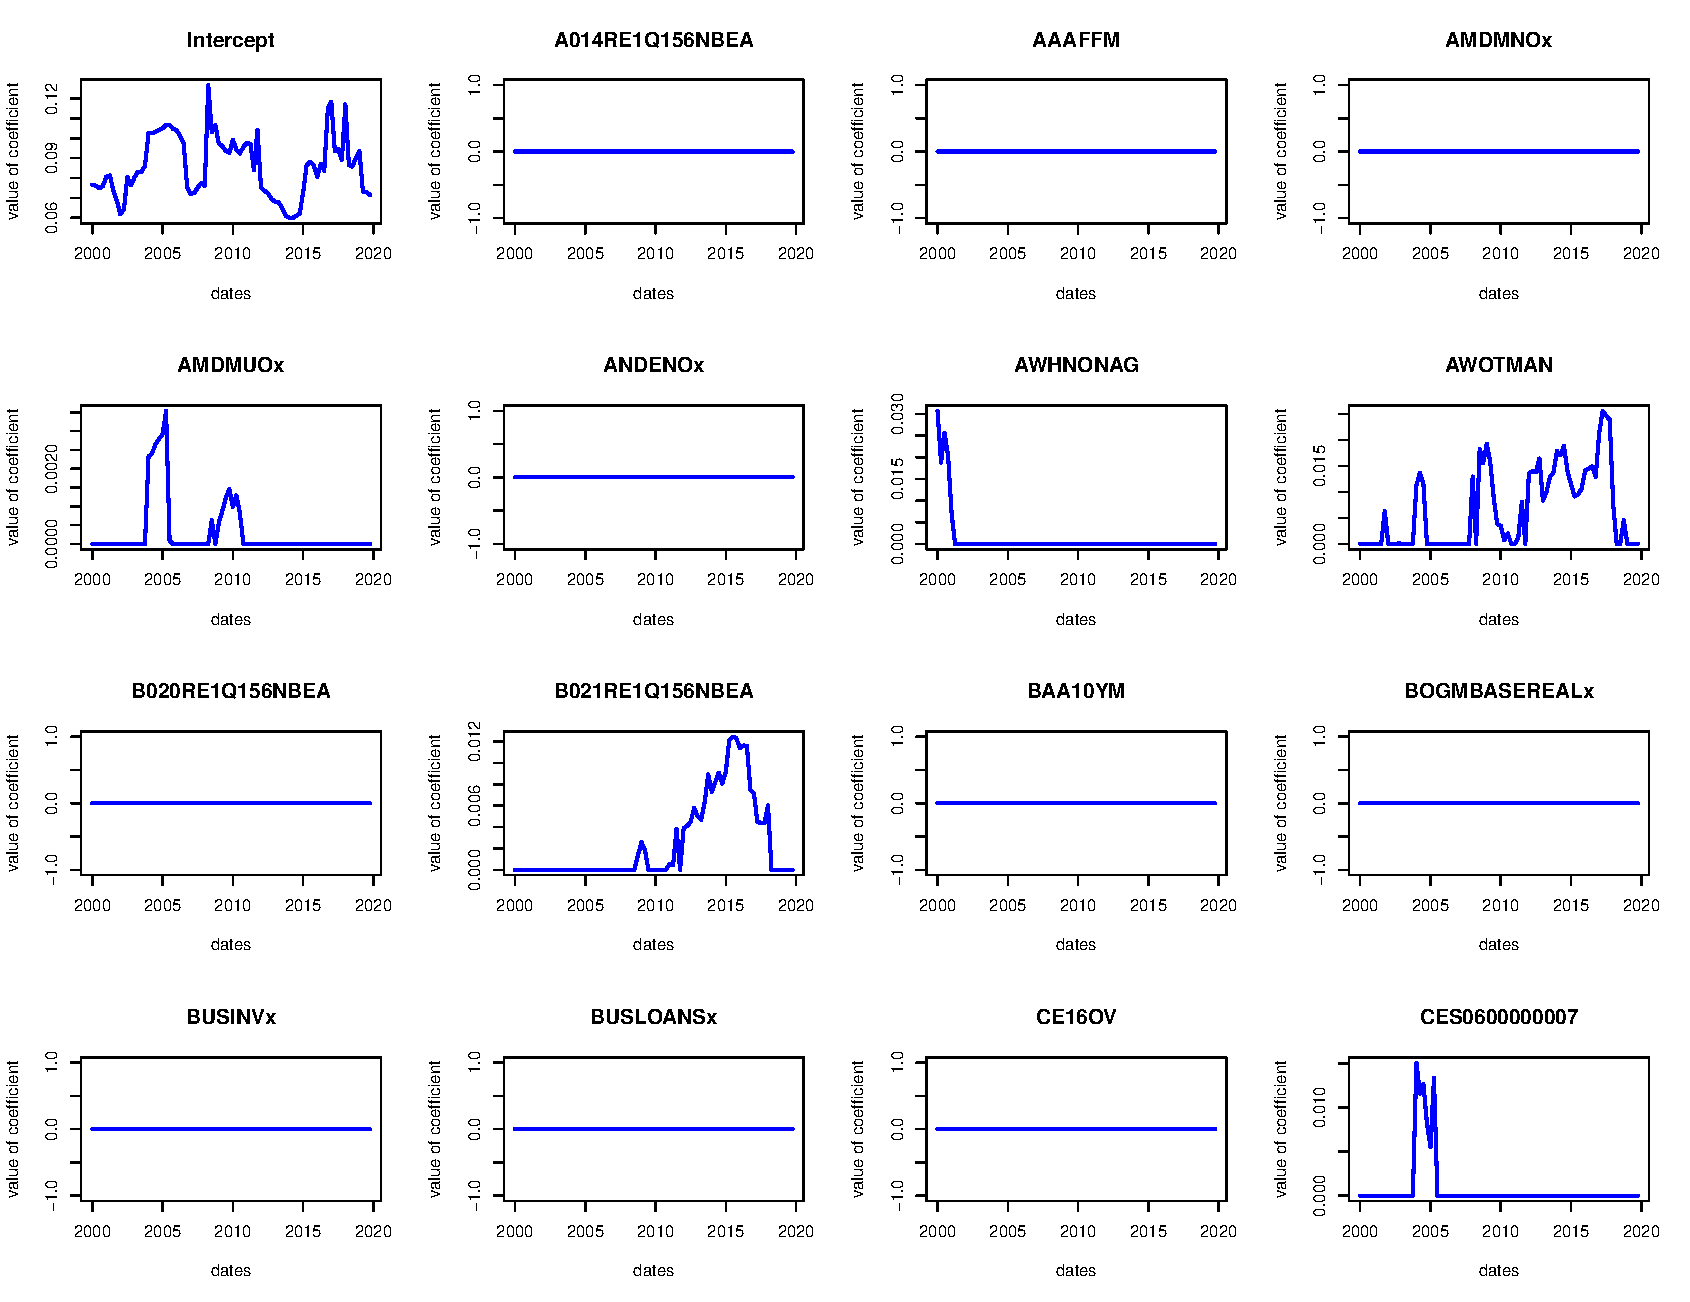
\includegraphics[page = 1, width=\textwidth]{plots/lasso_betas}
\label{fig:lasso_betas}
\caption{\label{first}Lasso regression: The evolution of the estimated $\beta$ coefficients over time}
\centering
\end{figure}

\begin{figure}[hbt!]
\includegraphics[page = 2, width=\textwidth]{plots/lasso_betas}
\label{fig:lasso_betas}
\caption{\label{second}Lasso regression: The evolution of the estimated $\beta$ coefficients over time}
\centering
\end{figure}

\begin{figure}[hbt!]
\includegraphics[page = 3, width=\textwidth]{plots/lasso_betas}
\label{fig:lasso_betas}
\caption{\label{third}Lasso regression: The evolution of the estimated $\beta$ coefficients over time}
\centering
\end{figure}

\begin{figure}[hbt!]
\includegraphics[page = 4, width=\textwidth]{plots/lasso_betas}
\label{fig:lasso_betas}
\caption{\label{fourth}Lasso regression: The evolution of the estimated $\beta$ coefficients over time}
\centering
\end{figure}

\begin{figure}[hbt!]
\includegraphics[page = 5, width=\textwidth]{plots/lasso_betas}
\label{fig:lasso_betas}
\caption{\label{fifth}Lasso regression: The evolution of the estimated $\beta$ coefficients over time}
\centering
\end{figure}

\begin{figure}[hbt!]
\includegraphics[page = 6, width=\textwidth]{plots/lasso_betas}
\label{fig:lasso_betas}
\caption{\label{sixth}Lasso regression: The evolution of the estimated $\beta$ coefficients over time}
\centering
\end{figure}

\begin{figure}[hbt!]
\includegraphics[page = 7, width=\textwidth]{plots/lasso_betas}
\label{fig:lasso_betas}
\caption{\label{seventh}Lasso regression: The evolution of the estimated $\beta$ coefficients over time}
\centering
\end{figure}

\begin{figure}[hbt!]
\includegraphics[page = 8, width=\textwidth]{plots/lasso_betas}
\label{fig:lasso_betas}
\caption{\label{eighth}Lasso regression: The evolution of the estimated $\beta$ coefficients over time}
\centering
\end{figure}

\begin{figure}[hbt!]
\includegraphics[page = 9, width=\textwidth]{plots/lasso_betas}
\label{fig:lasso_betas}
\caption{\label{ninth}Lasso regression: The evolution of the estimated $\beta$ coefficients over time}
\centering
\end{figure}

\begin{figure}[hbt!]
\includegraphics[page = 10, width=\textwidth]{plots/lasso_betas}
\label{fig:lasso_betas}
\caption{\label{tenth}Lasso regression: The evolution of the estimated $\beta$ coefficients over time}
\centering
\end{figure}

\begin{figure}[hbt!]
\includegraphics[page = 11, width=\textwidth]{plots/lasso_betas}
\label{fig:lasso_betas}
\caption{\label{eleventh}Lasso regression: The evolution of the estimated $\beta$ coefficients over time}
\centering
\end{figure}

\begin{figure}[hbt!]
\includegraphics[page = 12, width=\textwidth]{plots/lasso_betas}
\label{fig:lasso_betas}
\caption{\label{twelveth}Lasso regression: The evolution of the estimated $\beta$ coefficients over time}
\centering
\end{figure}

\begin{figure}[hbt!]
\includegraphics[page = 13, width=\textwidth]{plots/lasso_betas}
\label{fig:lasso_betas}
\caption{\label{thirteenth}Lasso regression: The evolution of the estimated $\beta$ coefficients over time}
\centering
\end{figure}

\end{subfigures}

\clearpage

\subsubsection{PCA}

\begin{subfigures}
\begin{figure}[hbt!]
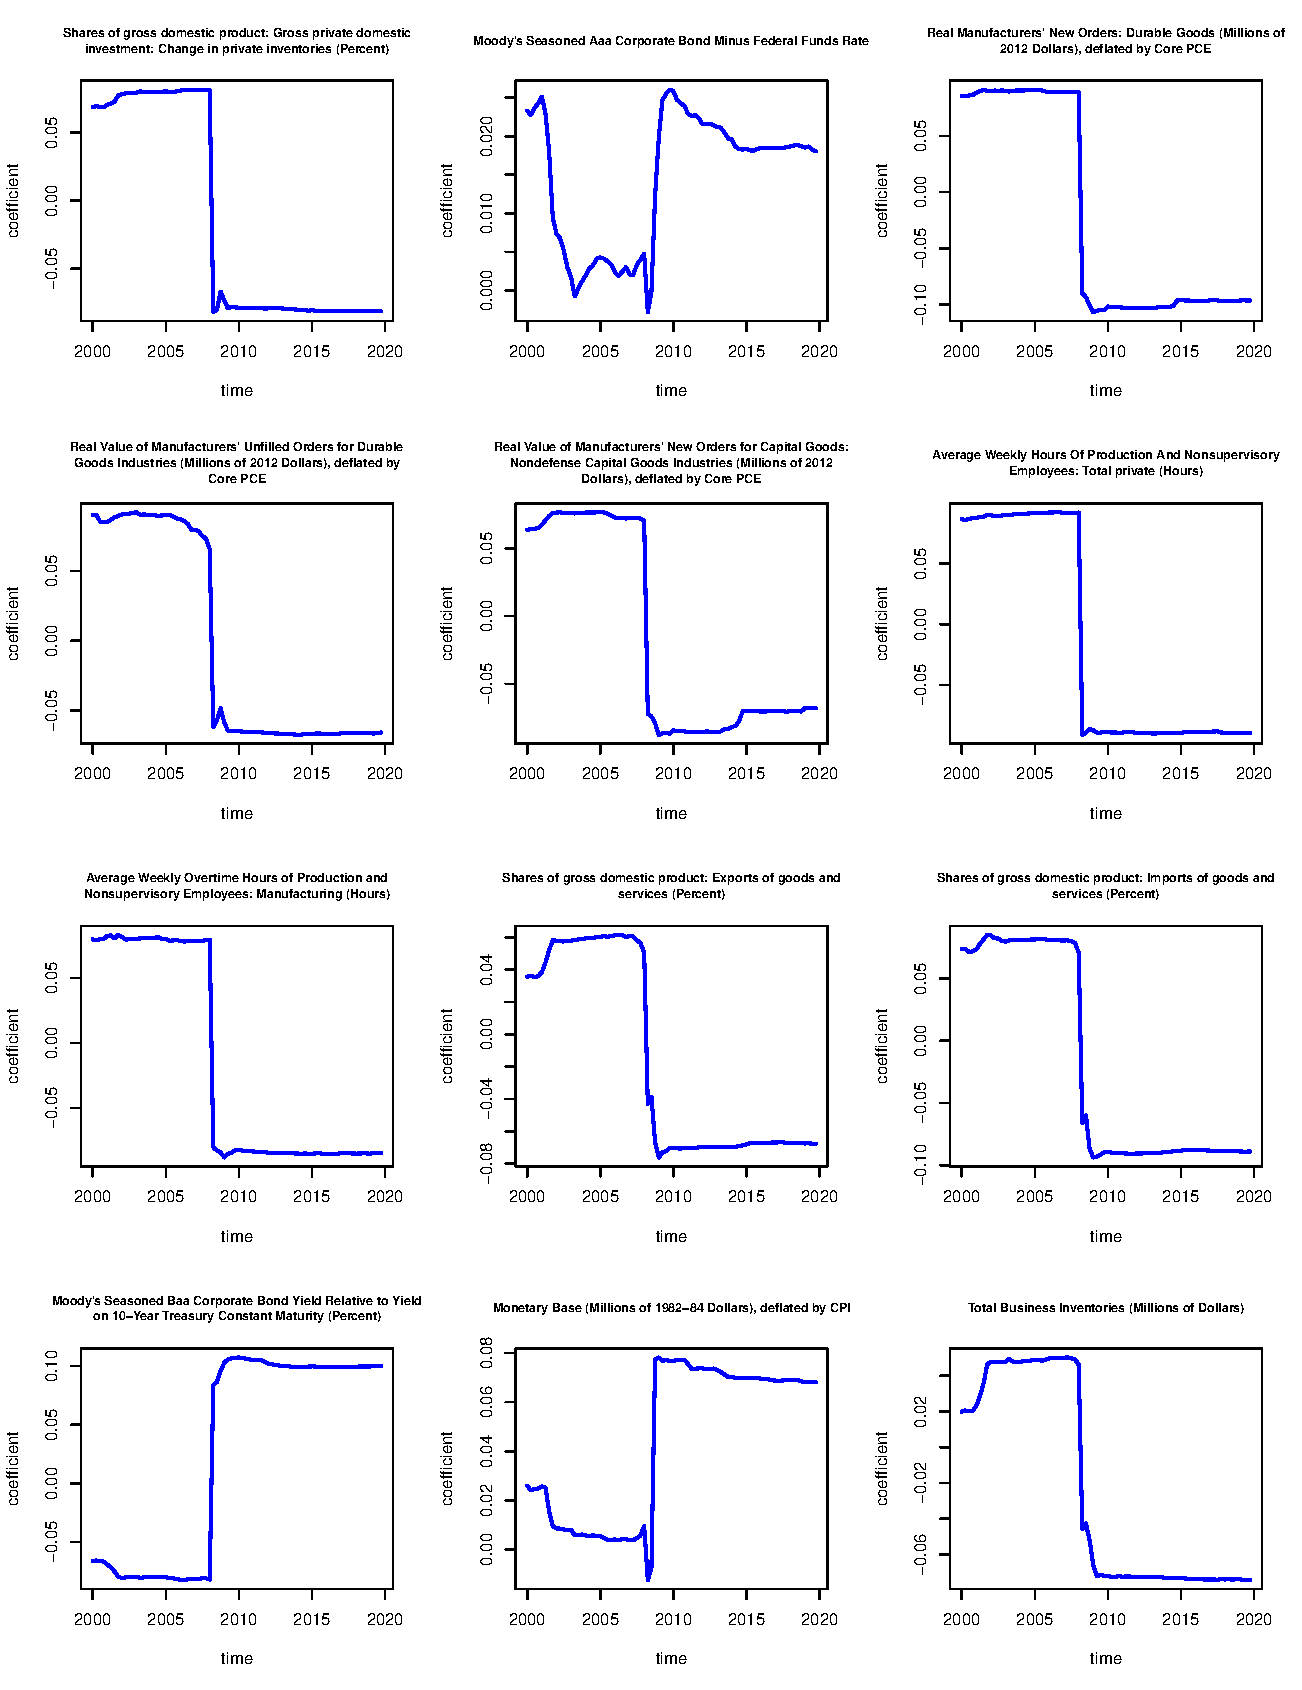
\includegraphics[page = 1, width=\textwidth]{plots/pca_loads}
\label{fig:pca_loads}
\caption{\label{first}PCA: The evolution of the loading factors over time}
\centering
\end{figure}

\begin{figure}[hbt!]
\includegraphics[page = 2, width=\textwidth]{plots/pca_loads}
\label{fig:pca_loads}
\caption{\label{second}PCA: The evolution of the loading factors over time}
\centering
\end{figure}

\begin{figure}[hbt!]
\includegraphics[page = 3, width=\textwidth]{plots/pca_loads}
\label{fig:pca_loads}
\caption{\label{third}PCA: The evolution of the loading factors over time}
\centering
\end{figure}

\begin{figure}[hbt!]
\includegraphics[page = 4, width=\textwidth]{plots/pca_loads}
\label{fig:pca_loads}
\caption{\label{fourth}PCA: The evolution of the loading factors over time}
\centering
\end{figure}

\begin{figure}[hbt!]
\includegraphics[page = 5, width=\textwidth]{plots/pca_loads}
\label{fig:pca_loads}
\caption{\label{fifth}PCA: The evolution of the loading factors over time}
\centering
\end{figure}

\begin{figure}[hbt!]
\includegraphics[page = 6, width=\textwidth]{plots/pca_loads}
\label{fig:pca_loads}
\caption{\label{sixth}PCA: The evolution of the loading factors over time}
\centering
\end{figure}

\begin{figure}[hbt!]
\includegraphics[page = 7, width=\textwidth]{plots/pca_loads}
\label{fig:pca_loads}
\caption{\label{seventh}PCA: The evolution of the loading factors over time}
\centering
\end{figure}

\begin{figure}[hbt!]
\includegraphics[page = 8, width=\textwidth]{plots/pca_loads}
\label{fig:pca_loads}
\caption{\label{eighth}PCA: The evolution of the loading factors over time}
\centering
\end{figure}

\begin{figure}[hbt!]
\includegraphics[page = 9, width=\textwidth]{plots/pca_loads}
\label{fig:pca_loads}
\caption{\label{ninth}PCA: The evolution of the loading factors over time}
\centering
\end{figure}

\begin{figure}[hbt!]
\includegraphics[page = 10, width=\textwidth]{plots/pca_loads}
\label{fig:pca_loads}
\caption{\label{tenth}PCA: The evolution of the loading factors over time}
\centering
\end{figure}

\begin{figure}[hbt!]
\includegraphics[page = 11, width=\textwidth]{plots/pca_loads}
\label{fig:pca_loads}
\caption{\label{eleventh}PCA: The evolution of the loading factors over time}
\centering
\end{figure}

\begin{figure}[hbt!]
\includegraphics[page = 12, width=\textwidth]{plots/pca_loads}
\label{fig:pca_loads}
\caption{\label{twelveth}PCA: The evolution of the loading factors over time}
\centering
\end{figure}

\begin{figure}[hbt!]
\includegraphics[page = 13, width=\textwidth]{plots/pca_loads}
\label{fig:pca_loads}
\caption{\label{thirteenth}PCA: The evolution of the loading factors over time}
\centering
\end{figure}

\end{subfigures}

\clearpage

\clearpage
\subsubsection{PLS}

\begin{subfigures}
\begin{figure}[hbt!]
\includegraphics[page = 1, width=\textwidth]{plots/pls_loads}
\label{fig:pls_loads}
\caption{\label{first}PLS: The evolution of the loading factors over time}
\centering
\end{figure}

\begin{figure}[hbt!]
\includegraphics[page = 2, width=\textwidth]{plots/pls_loads}
\label{fig:pls_loads}
\caption{\label{second}PLS: The evolution of the loading factors over time}
\centering
\end{figure}

\begin{figure}[hbt!]
\includegraphics[page = 3, width=\textwidth]{plots/pls_loads}
\label{fig:pls_loads}
\caption{\label{third}PLS: The evolution of the loading factors over time}
\centering
\end{figure}

\begin{figure}[hbt!]
\includegraphics[page = 4, width=\textwidth]{plots/pls_loads}
\label{fig:pls_loads}
\caption{\label{fourth}PLS: The evolution of the loading factors over time}
\centering
\end{figure}

\begin{figure}[hbt!]
\includegraphics[page = 5, width=\textwidth]{plots/pls_loads}
\label{fig:pls_loads}
\caption{\label{fifth}PLS: The evolution of the loading factors over time}
\centering
\end{figure}

\begin{figure}[hbt!]
\includegraphics[page = 6, width=\textwidth]{plots/pls_loads}
\label{fig:pls_loads}
\caption{\label{sixth}PLS: The evolution of the loading factors over time}
\centering
\end{figure}

\begin{figure}[hbt!]
\includegraphics[page = 7, width=\textwidth]{plots/pls_loads}
\label{fig:pls_loads}
\caption{\label{seventh}PLS: The evolution of the loading factors over time}
\centering
\end{figure}

\begin{figure}[hbt!]
\includegraphics[page = 8, width=\textwidth]{plots/pls_loads}
\label{fig:pls_loads}
\caption{\label{eighth}PLS: The evolution of the loading factors over time}
\centering
\end{figure}

\begin{figure}[hbt!]
\includegraphics[page = 9, width=\textwidth]{plots/pls_loads}
\label{fig:pls_loads}
\caption{\label{ninth}PLS: The evolution of the loading factors over time}
\centering
\end{figure}

\begin{figure}[hbt!]
\includegraphics[page = 10, width=\textwidth]{plots/pls_loads}
\label{fig:pls_loads}
\caption{\label{tenth}PLS: The evolution of the loading factors over time}
\centering
\end{figure}

\begin{figure}[hbt!]
\includegraphics[page = 11, width=\textwidth]{plots/pls_loads}
\label{fig:pls_loads}
\caption{\label{eleventh}PLS: The evolution of the loading factors over time}
\centering
\end{figure}

\begin{figure}[hbt!]
\includegraphics[page = 12, width=\textwidth]{plots/pls_loads}
\label{fig:pls_loads}
\caption{\label{twelveth}PLS: The evolution of the loading factors over time}
\centering
\end{figure}

\begin{figure}[hbt!]
\includegraphics[page = 13, width=\textwidth]{plots/pls_loads}
\label{fig:pls_loads}
\caption{\label{thirteenth}PLS: The evolution of the loading factors over time}
\centering
\end{figure}

\end{subfigures}

\clearpage

\clearpage




\end{document}
